\documentclass{standalone}

\usepackage{tikz}
\usetikzlibrary{arrows}
\usetikzlibrary{decorations.markings}
\usetikzlibrary{calc}

\definecolor{lightblue}{RGB}{124,190,255}
\definecolor{darkgreen}{RGB}{24,145,0}

\begin{document}

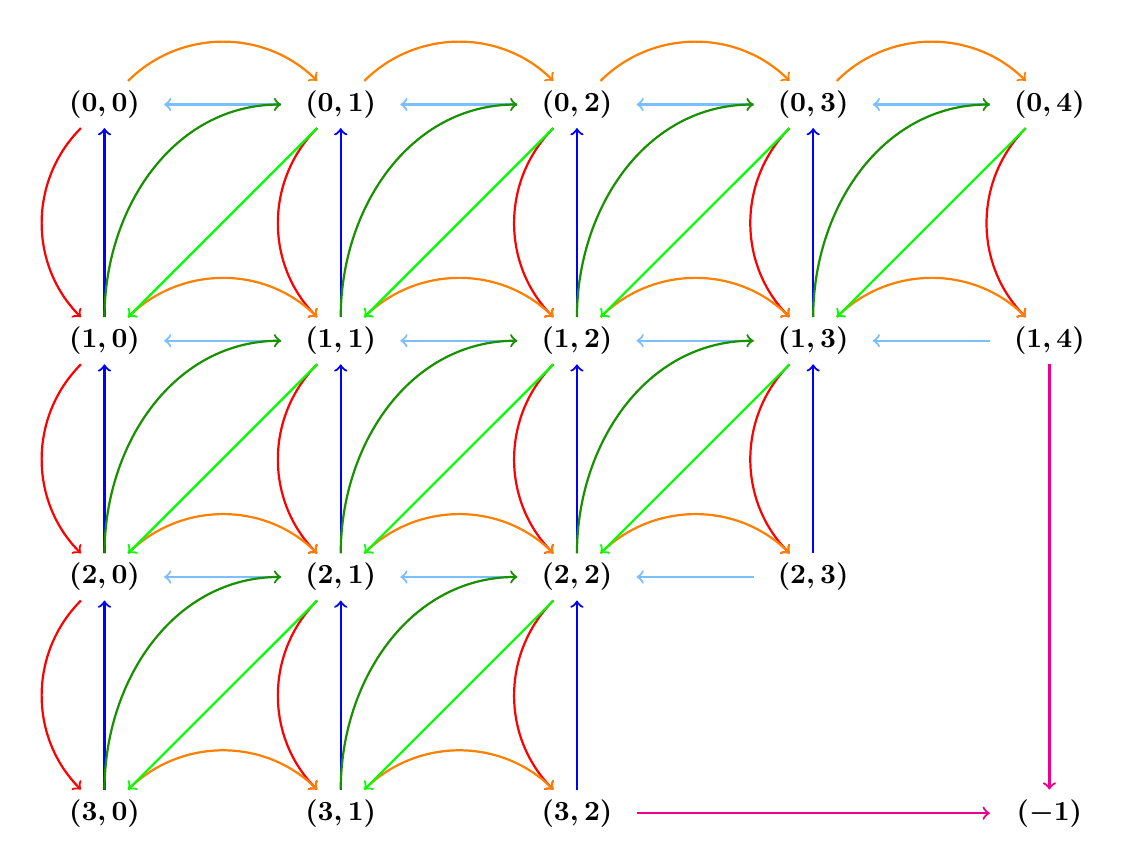
\begin{tikzpicture}
    \tikzstyle{state}=[minimum width=1.5cm, font=\boldmath];
    % First row
    \node (00) at (0,0) [state] {$(0,0)$};
    \node (01) at ($(00)+(3,0)$) [state] {$(0,1)$};
    \node (02) at ($(01)+(3,0)$) [state] {$(0,2)$};
    \node (03) at ($(02)+(3,0)$) [state] {$(0,3)$};
    \node (04) at ($(03)+(3,0)$) [state] {$(0,4)$};

    % Second row
    \node (10) at ($(00)+(0,-3)$) [state] {$(1,0)$};
    \node (11) at ($(10)+(3,0)$) [state] {$(1,1)$};
    \node (12) at ($(11)+(3,0)$) [state] {$(1,2)$};
    \node (13) at ($(12)+(3,0)$) [state] {$(1,3)$};
    \node (14) at ($(13)+(3,0)$) [state] {$(1,4)$};

    % Third row
    \node (20) at ($(10)+(0,-3)$) [state] {$(2,0)$};
    \node (21) at ($(20)+(3,0)$) [state] {$(2,1)$};
    \node (22) at ($(21)+(3,0)$) [state] {$(2,2)$};
    \node (23) at ($(22)+(3,0)$) [state] {$(2,3)$};

    % Fourth row
    \node (30) at ($(20)+(0,-3)$) [state] {$(3,0)$};
    \node (31) at ($(30)+(3,0)$) [state] {$(3,1)$};
    \node (32) at ($(31)+(3,0)$) [state] {$(3,2)$};

    \node (-1) at ($(32)+(6,0)$) [state] {$(-1)$};

    % Transitions
    % Arrivals
    \draw[red] (00) edge[out=-135,in=135,->,thick] (10);
    \draw[red] (01) edge[out=-135,in=135,->,thick] (11);
    \draw[red] (02) edge[out=-135,in=135,->,thick] (12);
    \draw[red] (03) edge[out=-135,in=135,->,thick] (13);
    \draw[red] (04) edge[out=-135,in=135,->,thick] (14);

    \draw[red] (10) edge[out=-135,in=135,->,thick] (20);
    \draw[red] (11) edge[out=-135,in=135,->,thick] (21);
    \draw[red] (12) edge[out=-135,in=135,->,thick] (22);
    \draw[red] (13) edge[out=-135,in=135,->,thick] (23);

    \draw[red] (20) edge[out=-135,in=135,->,thick] (30);
    \draw[red] (21) edge[out=-135,in=135,->,thick] (31);
    \draw[red] (22) edge[out=-135,in=135,->,thick] (32);

    \draw[orange] (00) edge[out=45,in=135,->,thick] (01);
    \draw[orange] (01) edge[out=45,in=135,->,thick] (02);
    \draw[orange] (02) edge[out=45,in=135,->,thick] (03);
    \draw[orange] (03) edge[out=45,in=135,->,thick] (04);

    \draw[orange] (10) edge[out=45,in=135,->,thick] (11);
    \draw[orange] (11) edge[out=45,in=135,->,thick] (12);
    \draw[orange] (12) edge[out=45,in=135,->,thick] (13);
    \draw[orange] (13) edge[out=45,in=135,->,thick] (14);

    \draw[orange] (20) edge[out=45,in=135,->,thick] (21);
    \draw[orange] (21) edge[out=45,in=135,->,thick] (22);
    \draw[orange] (22) edge[out=45,in=135,->,thick] (23);

    \draw[orange] (30) edge[out=45,in=135,->,thick] (31);
    \draw[orange] (31) edge[out=45,in=135,->,thick] (32);

    % % First Station Service and exit
    \draw[blue] (00) edge[<-,thick] (10);
    \draw[blue] (01) edge[<-,thick] (11);
    \draw[blue] (02) edge[<-,thick] (12);
    \draw[blue] (03) edge[<-,thick] (13);

    \draw[blue] (10) edge[<-,thick] (20);
    \draw[blue] (11) edge[<-,thick] (21);
    \draw[blue] (12) edge[<-,thick] (22);
    \draw[blue] (13) edge[<-,thick] (23);

    \draw[blue] (20) edge[<-,thick] (30);
    \draw[blue] (21) edge[<-,thick] (31);
    \draw[blue] (22) edge[<-,thick] (32);

    % Second station service and exit
    \draw[lightblue] (04) edge[->,thick] (03);
    \draw[lightblue] (03) edge[->,thick] (02);
    \draw[lightblue] (02) edge[->,thick] (01);
    \draw[lightblue] (01) edge[->,thick] (00);

    \draw[lightblue] (14) edge[->,thick] (13);
    \draw[lightblue] (13) edge[->,thick] (12);
    \draw[lightblue] (12) edge[->,thick] (11);
    \draw[lightblue] (11) edge[->,thick] (10);

    \draw[lightblue] (23) edge[->,thick] (22);
    \draw[lightblue] (22) edge[->,thick] (21);
    \draw[lightblue] (21) edge[->,thick] (20);

    % 1st station service and transition
    \draw[darkgreen] (30) edge[out=90,in=180,->,thick] (21);
    \draw[darkgreen] (20) edge[out=90,in=180,->,thick] (11);
    \draw[darkgreen] (10) edge[out=90,in=180,->,thick] (01);

    \draw[darkgreen] (31) edge[out=90,in=180,->,thick] (22);
    \draw[darkgreen] (21) edge[out=90,in=180,->,thick] (12);
    \draw[darkgreen] (11) edge[out=90,in=180,->,thick] (02);

    \draw[darkgreen] (22) edge[out=90,in=180,->,thick] (13);
    \draw[darkgreen] (12) edge[out=90,in=180,->,thick] (03);

    \draw[darkgreen] (13) edge[out=90,in=180,->,thick] (04);

    % 2ns station service and transition
    \draw[green] (21) edge[->,thick] (30);
    \draw[green] (11) edge[->,thick] (20);
    \draw[green] (01) edge[->,thick] (10);

    \draw[green] (22) edge[->,thick] (31);
    \draw[green] (12) edge[->,thick] (21);
    \draw[green] (02) edge[->,thick] (11);

    \draw[green] (13) edge[->,thick] (22);
    \draw[green] (03) edge[->,thick] (12);

    \draw[green] (04) edge[->,thick] (13);

    % To deadlock
    \draw[magenta] (14) edge[->,thick] (-1);
    \draw[magenta] (32) edge[->,thick] (-1);


\end{tikzpicture}

\end{document}
